% Created 2022-09-16 Fri 10:13
% Intended LaTeX compiler: xelatex
\documentclass[aspectratio=1610,xcolor={dvipsnames},hyperref={colorlinks,unicode,linkcolor=violet,anchorcolor=blueviolet,citecolor=YellowOrange,filecolor=black,urlcolor=Aquamarine}]{beamer}
\usepackage{graphicx}
\usepackage{grffile}
\usepackage{longtable}
\usepackage{booktabs}
\usepackage{wrapfig}
\usepackage{rotating}
\usepackage[normalem]{ulem}
\usepackage{amsmath}
\usepackage{textcomp}
\usepackage{amssymb}
\usepackage{capt-of}
\usepackage{nicefrac}
\usepackage[dvipsnames]{xcolor}
\usepackage[colorlinks,unicode,linkcolor=violet,anchorcolor=blueviolet,citecolor=YellowOrange,filecolor=black,urlcolor=Aquamarine]{hyperref}
\usepackage{listings}
\usepackage{etoolbox}
\useoutertheme{infolines}
\setbeamertemplate{frametitle}{%
\usebeamerfont{frametitle}\insertframetitle\strut%
\vskip-0\baselineskip%
\leaders\vrule width .95\paperwidth\vskip1pt%
\vskip0pt%
\nointerlineskip
}

%% T for footer
\setbeamercolor{footlinecolor}{fg=cyan,bg=green}
\setbeamercolor{author in head/foot}{fg=blue}
\setbeamertemplate{footline}{%
\leavevmode%
\hbox{%
\begin{beamercolorbox}[wd=.26\paperwidth,ht=2.25ex,dp=1ex,left]{author in head/foot}%
\hspace*{2ex}\usebeamerfont{author in head/foot} Dept. CSE, UT Arlington
\end{beamercolorbox}%
\begin{beamercolorbox}[wd=.50\paperwidth,ht=2.25ex,dp=1ex,center]{author in head/foot}%
\usebeamerfont{title in head/foot}Scalable Modeling \& Imaging \& Learning Lab (SMILE)
\end{beamercolorbox}%
\begin{beamercolorbox}[wd=.24\paperwidth,ht=2.25ex,dp=1ex,right]{date in head/foot}%
\usebeamerfont{date in head/foot}
\insertshortdate{}\hspace*{1em}  % date
\insertframenumber/\inserttotalframenumber\hspace*{2ex}
\end{beamercolorbox}}%
\vskip0pt%
}
\setbeamerfont{footnote}{size=\tiny}
\usetheme{default}
\usefonttheme{serif}
\useinnertheme{circles}
\author{Nasy}
\date{Sep 16, 2022}
\title{T-Cell Receptor-Peptide Interaction Prediction with Physical Model Augmented Pseudo-Labeling}
\hypersetup{
 pdfauthor={Nasy},
 pdftitle={T-Cell Receptor-Peptide Interaction Prediction with Physical Model Augmented Pseudo-Labeling},
 pdfkeywords={},
 pdfsubject={},
 pdfcreator={Emacs 29.0.50 (Org mode 9.5.4)}, 
 pdflang={English}}
\usepackage[style=mla]{biblatex}
\addbibresource{~/.emacs.d/萚兮/旹/refs/ref.bib}
\begin{document}

\maketitle
\begin{frame}{Outline}
\tableofcontents
\end{frame}


\section{Introduction}
\label{sec:org262cdd8}

\begin{frame}[label={sec:org7383039}]{TCR Peptide Interaction Prediction}
\begin{columns}
\begin{column}{0.4\columnwidth}
\begin{block}{TCR Peptide Interaction}
\begin{itemize}
\item The T-cell receptors (TCR) lies on the surface of the T-cell for recognition of foreign peptides.
\item Peptides are presented by major histocompatibility complex (MHC) found on the surface of tumor cells or virus-infected cells.
\item Common datasets for studying TCR-peptide interactions contain sequences of peptides and sequences of 𝛽 chain of CDR3 of TCRs.
\end{itemize}
\end{block}
\end{column}

\begin{column}{0.4\columnwidth}
\begin{block}{Illustration of T-cell receptors (TCR) and peptide binding}
\begin{center}
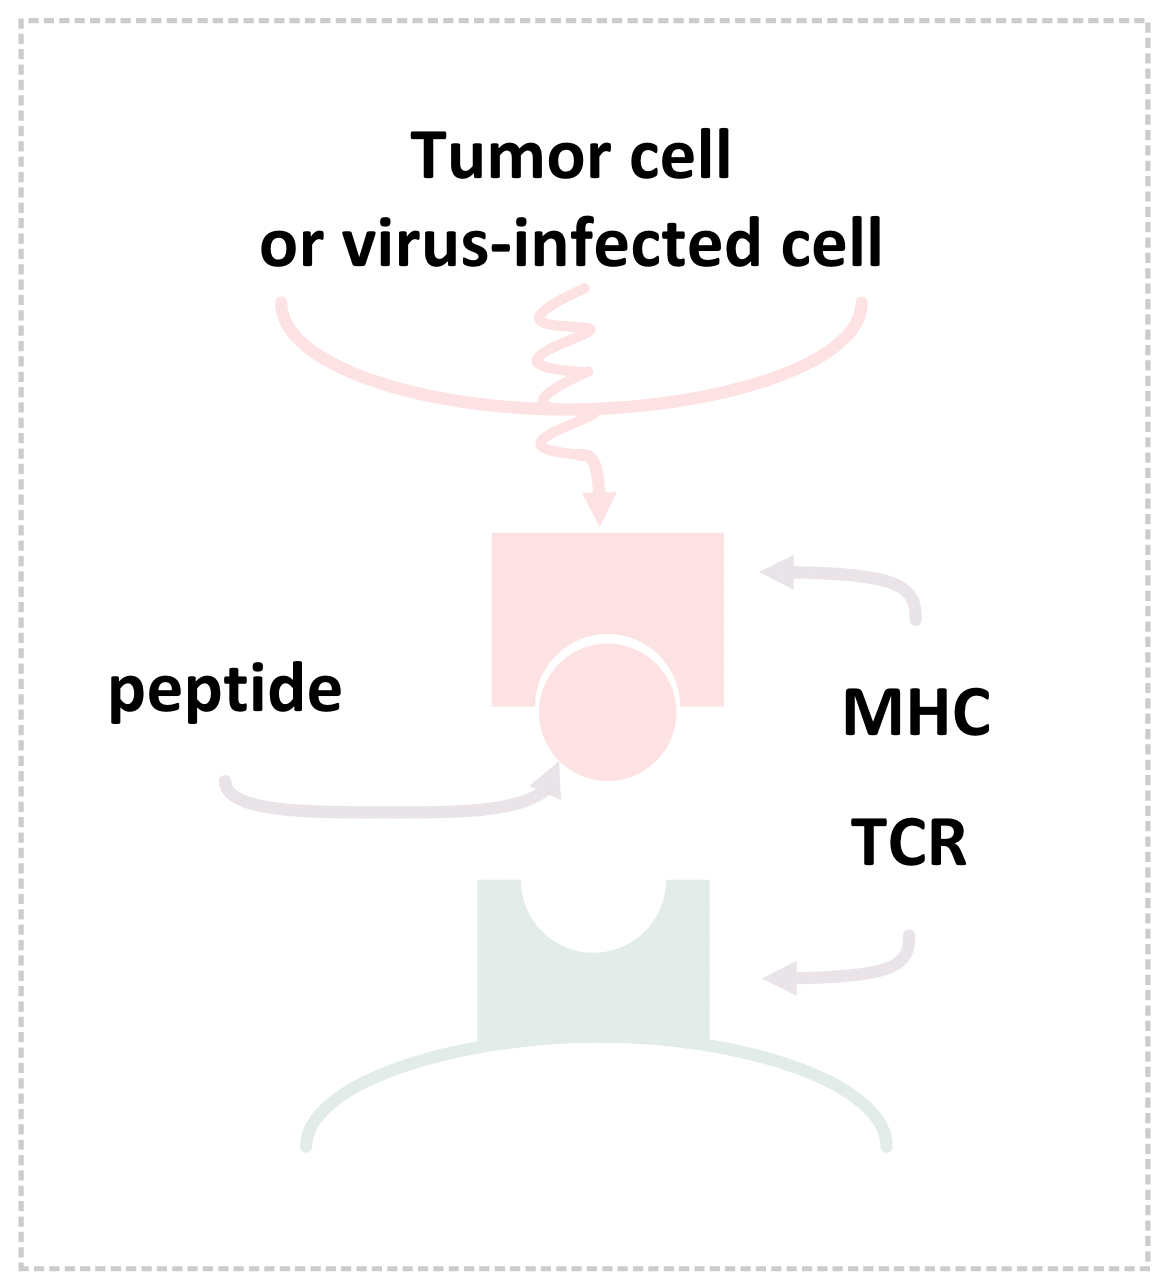
\includegraphics[width=.9\linewidth]{./p1.png}
\end{center}
\end{block}
\end{column}
\end{columns}
\end{frame}

\begin{frame}[label={sec:org55d3065}]{Methods}
\begin{itemize}
\item Nearest neighbor (SwarmTCR \footfullcite{ehrlichSwarmTCRComputationalApproach2021})
\item Distance-based minimization (TCRdist \footfullcite{dashQuantifiablePredictiveFeatures2017})
\item PCA with decision tree \footfullcite{tongSETESequencebasedEnsemble2020}
\item Random Forest \footfullcite{gielisDetectionEnrichedCell2019a,deneuterFeasibilityMiningCD82018}
\item Deep Learning \footfullcite{luDeepLearningbasedPrediction2021,jianTCellReceptorPeptideInteraction2022}
\end{itemize}
\end{frame}

\begin{frame}[label={sec:org70c4332}]{Datasets}
\begin{itemize}
\item Format
\begin{itemize}
\item Positive (TCR, Peptide, MHC)
\item And lots of TCRs
\end{itemize}
\item Dataset
\begin{itemize}
\item VDJdb \footfullcite{bagaevVDJdb2019Database2020}
\item McPAS-TCR \footfullcite{tickotskyMcPASTCRManuallyCurated2017}
\end{itemize}
\end{itemize}
\end{frame}

\section{T-Cell Receptor-Peptide Interaction Prediction with Physical Model Augmented Pseudo-Labeling}
\label{sec:org4758d7b}

\begin{frame}[label={sec:orgd7716ec}]{Paper}
\begin{center}
\LARGE T-Cell Receptor-Peptide Interaction Prediction with Physical Model Augmented Pseudo-Labeling \normalsize \footfullcite{jianTCellReceptorPeptideInteraction2022}
\end{center}
\end{frame}

\begin{frame}[label={sec:org0a46d23}]{Problem}
\begin{center}
\Large Current datasets for training deep learning models of this purpose remain constrained without diverse TCRs and peptides.
\end{center}
\end{frame}

\begin{frame}[label={sec:orgea0d18d}]{Solution}
\begin{center}
\Large Extend training dataset
\end{center}
\end{frame}

\begin{frame}[label={sec:orgf452d1e}]{Solution}
\begin{itemize}
\item Data-augmented psudo-label of TCR-peptide pairs
\begin{itemize}
\item Use teacher model to generate pseudo-labels and retrain the model with them
\end{itemize}
\item Physical modeling of TCR-peptide interaction
\begin{itemize}
\item Molecular dynamic (MD)
\item Docking energy
\end{itemize}
\end{itemize}
\end{frame}

\begin{frame}[label={sec:orga9c8cd2}]{What is Docking energy}
Docking is a computational method for predicting the structures of
protein complex (e.g., dimer of two molecules) given the structure of
each monomer. It searches the configuration of the complex by
minimizing an energy scoring function.

In this work, they use the final docking energy (of the optimal
structure of the complex) between a TCR and peptide as the surrogate
binding label for the TCR-peptide pair.
\end{frame}

\begin{frame}[label={sec:orgba90bb2}]{Dataset}
\begin{itemize}
\item Dataset \(\mathcal{D}\)
\begin{itemize}
\item VDJdb \footfullcite{bagaevVDJdb2019Database2020}
\item McPAS-TCR \footfullcite{tickotskyMcPASTCRManuallyCurated2017}
\end{itemize}
\item Labeled (Training dataset, \(\mathcal{D}_{train}\))
\begin{itemize}
\item TCR-peptide pairs with known binding affinity (1 positive, 0 negative)
\end{itemize}
\item Unlabeled
\begin{itemize}
\item TCRdb (no peptide) with peptide from \(\mathcal{D}\).
\item \(\mathcal{D}_{auxiliary}\)
\end{itemize}
\end{itemize}
\end{frame}

\begin{frame}[label={sec:org47b6726}]{Method}
There are four steps in a single training step:

\begin{itemize}
\item Learning from labeled dataset \(\mathcal{L}_{label}\)
\item Learning from physical modeling \(\mathcal{L}_{phy}\)
\item Learning from data-augmented pseudo-labeling \(\mathcal{L}_{pseudo-label}\)
\item Look ahead meta-update
\end{itemize}

\begin{columns}
\begin{column}{0.4\columnwidth}
\begin{block}{Overview}
\begin{center}
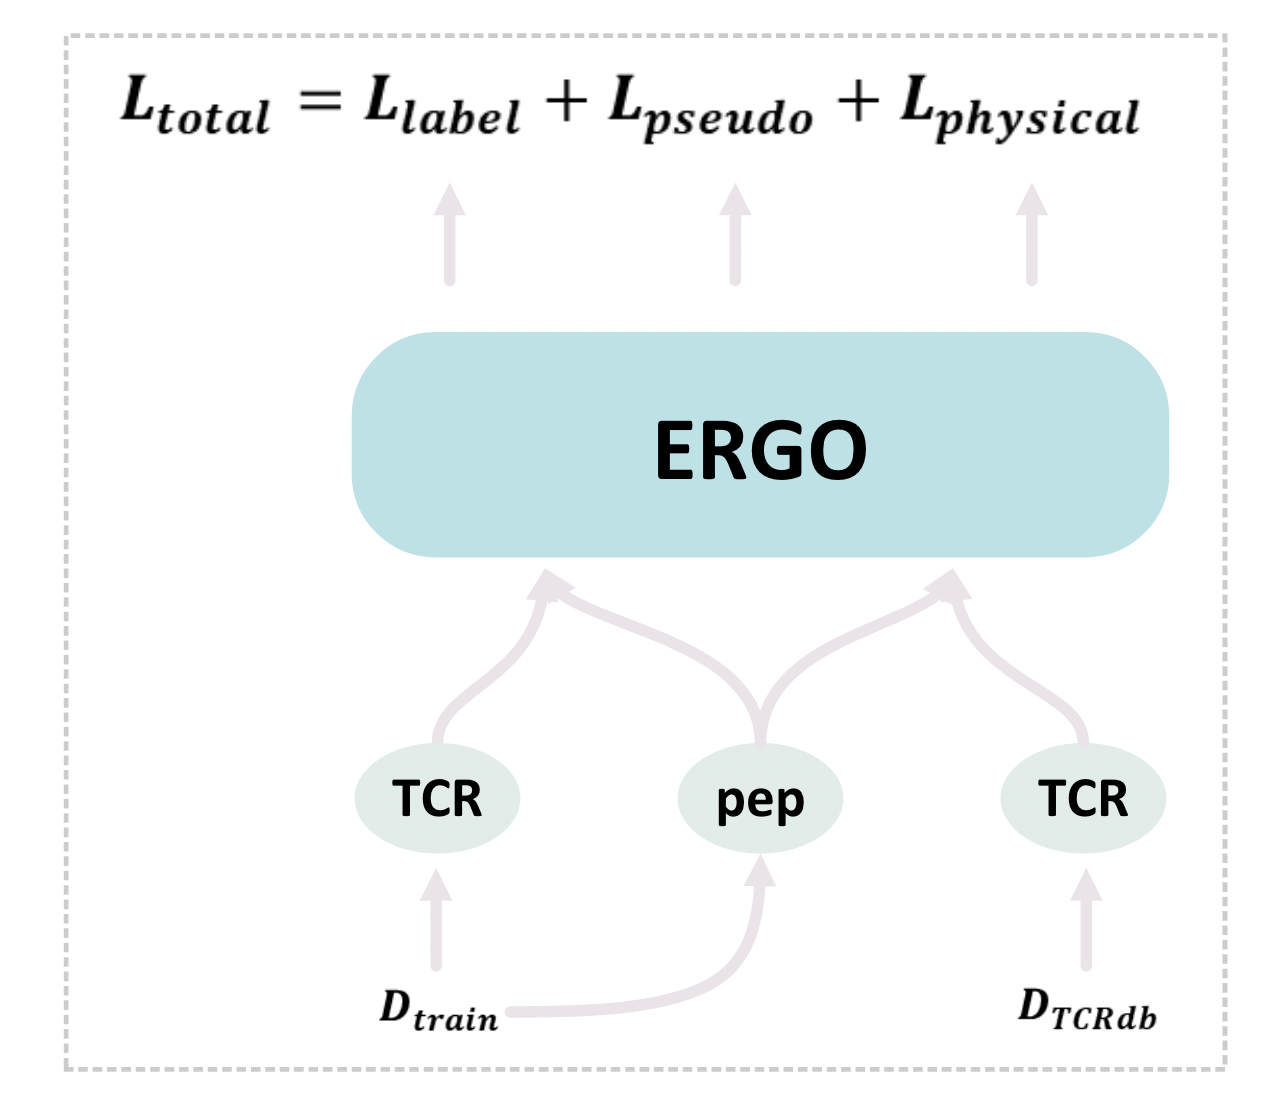
\includegraphics[width=.9\linewidth]{./p2.png}
\end{center}
\end{block}
\end{column}

\begin{column}{0.4\columnwidth}
\begin{block}{ERGO}
\begin{center}
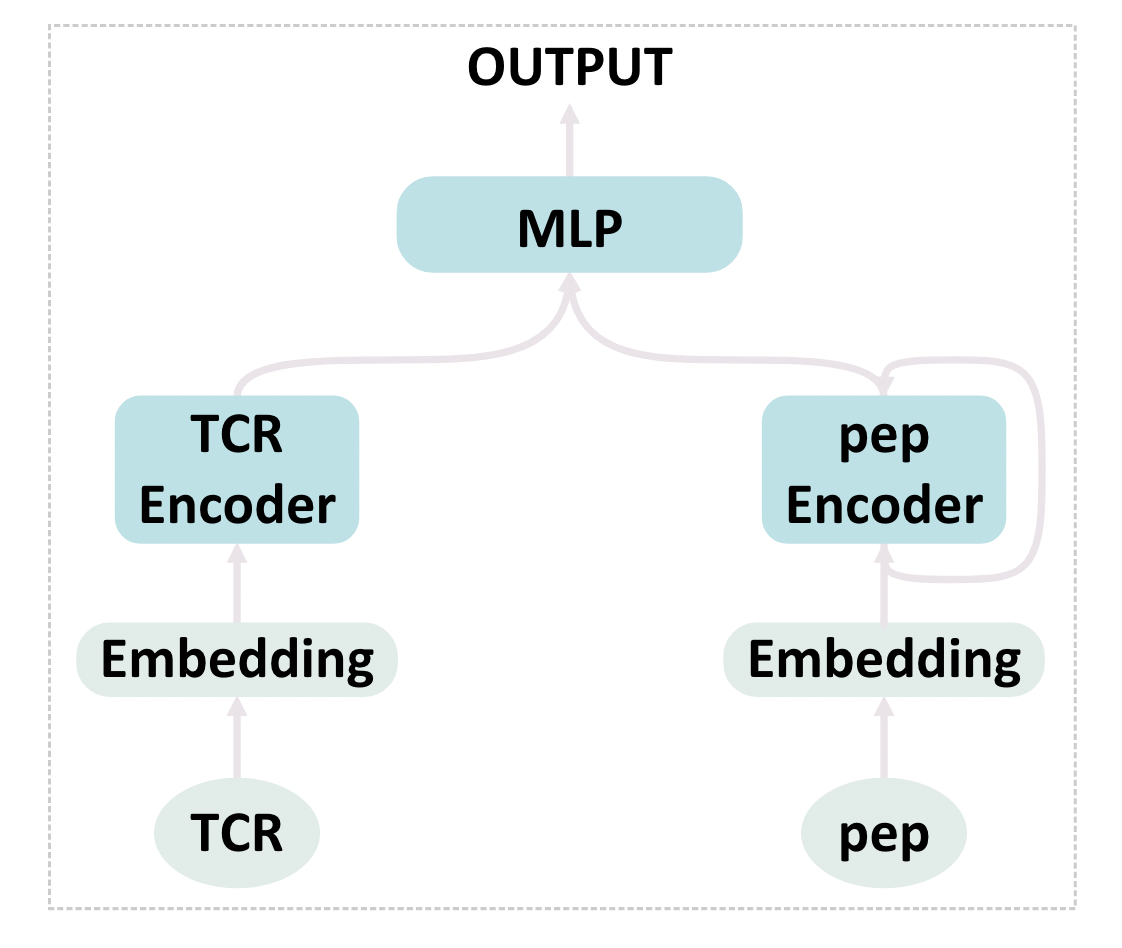
\includegraphics[width=.9\linewidth]{./p3.png}
\end{center}
\end{block}
\end{column}
\end{columns}
\end{frame}

\begin{frame}[label={sec:orgfbb2a02}]{Learning from labeled dataset \(\mathcal{L}_{label}\)}
\begin{itemize}
\item \(pred = f_{\theta}(t, p)\)
\begin{itemize}
\item \(t\) is the TCR
\item \(p\) is the peptide
\item The embedding of TCR and peptide from ERGO \footfullcite{springerPredictionSpecificTCRPeptide2020}.
\begin{itemize}
\item TCRs use LSTM or AE
\item Peptides use LSTM
\end{itemize}
\item \(f_{\theta}\) is the model
\begin{itemize}
\item \(f_{\theta} = MLP(concat(t, p))\)
\end{itemize}
\end{itemize}
\item \(\mathcal{L}_{label} = BCE(pred, y)\)
\end{itemize}
\end{frame}

\begin{frame}[label={sec:orgdb0a9c9}]{Learning from physical modeling \(\mathcal{L}_{phy}\)}
\begin{itemize}
\item Molecular dynamic (MD): accurate but slow
\item Docking energy: HDOCK \footfullcite{yanHDOCKServerIntegrated2020a}
\item TCR/Peptide -> BLAST+ -> MSA -> MODELLER -> Structure -> Docking energy
\begin{itemize}
\item Top 25\% Negative
\item Bottom 25\% Positive
\end{itemize}
\item \(pred' = f_{\theta}(t', p')\)
\begin{itemize}
\item \((t', p')\) become tuples in \(\mathcal{D}_{auxiliary}\)
\end{itemize}
\item \(\mathcal{L}_{phy} = BCE(pred', y)\)
\end{itemize}
\end{frame}

\begin{frame}[label={sec:org3b2b31a}]{Learning from data-augmented pseudo-labeling \(\mathcal{L}_{pseudo-label}\)}
\begin{itemize}
\item \(prob = f_{teacher}(t', p')\)
\item \(pred' = f_{\theta}(t', p')\)
\item \(\mathcal{L}_{pseudo-label} = \mathtt{KL-divergence}(pred', prob)\)
\end{itemize}
\end{frame}

\begin{frame}[allowframebreaks]{Look Ahead Meta-Update}
\begin{itemize}
\item Learning from labeled dataset
\begin{itemize}
\item \(out = model(t, p)\)
\item \(\mathcal{L}_{label} = BCE(out)\)
\item \(model.update(\mathcal{L}_{label})\)
\end{itemize}
\item Learning from data-augmented pseudo-labeling
\begin{itemize}
\item \(out = model(t', p')\)
\item \(out' = model_{teacher}(t', p')\)
\item \(\mathcal{L}_{pseudo-label} = KL(out, out')\)
\item \(model.update(\mathcal{L}_{pseudo-label})\)
\item \(param = model.param\)
\end{itemize}
\item Learning from physical modeling
\begin{itemize}
\item \(out = model(t', p')\)
\item \(\mathcal{L}_{phy} = BCE(out)\)
\item \(model.update(\mathcal{L}_{phy})\)
\end{itemize}
\item Look ahead meta-update
\begin{itemize}
\item Learning Rate * 2
\item \(\mathcal{L} = BCE(model(t, p))\)
\item If \(\mathcal{L} > \mathcal{L}_{label}\)
\begin{itemize}
\item \(model.param = param\)
\end{itemize}
\end{itemize}
\end{itemize}
\end{frame}

\begin{frame}[label={sec:org2213fc4}]{Look Ahead Meta-Update}
\begin{figure}[htbp]
\centering
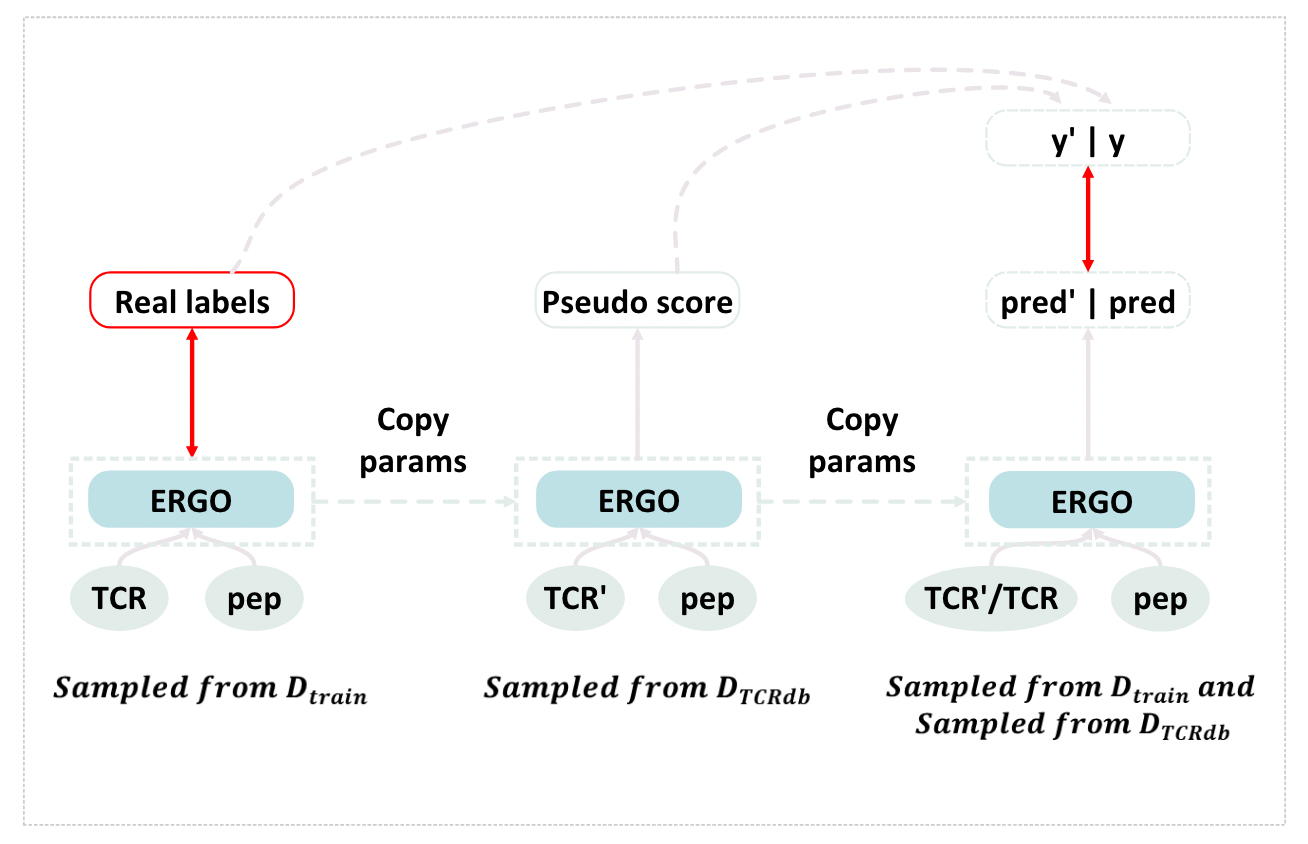
\includegraphics[height=5cm]{./pm.png}
\caption{\label{fig:org9dd8916}Overview of learning from data-augmented pseudolabeling. An ERGO model is first learned with TCRs and peptides sample from Dtrain, and this model is used as the teacher model. Then, this teacher model is used for pseudolabeling TCR-peptide pairs from auxiliary dataset. Finally, we re-train an ERGO model with the original dataset and the extended pseudo-labeled dataset.}
\end{figure}
\end{frame}

\begin{frame}[label={sec:orgde52991}]{Results McPAS}
\begin{columns}
\begin{column}{0.4\columnwidth}
\begin{block}{LSTM}
\begin{center}
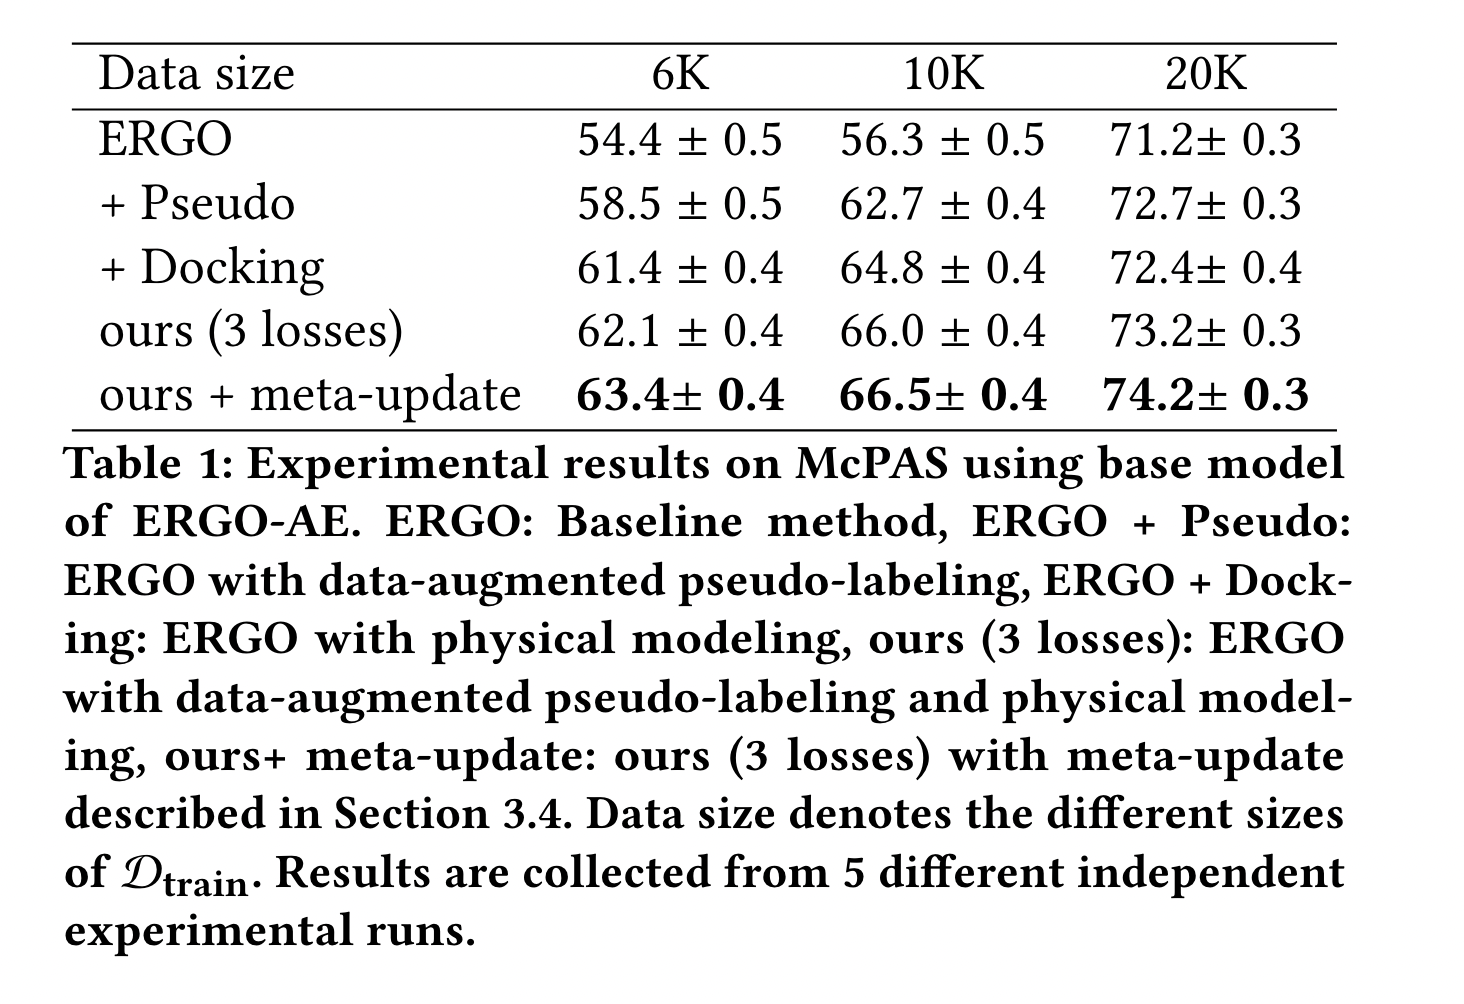
\includegraphics[width=.9\linewidth]{./p4.png}
\end{center}
\end{block}
\end{column}

\begin{column}{0.4\columnwidth}
\begin{block}{AE}
\begin{center}
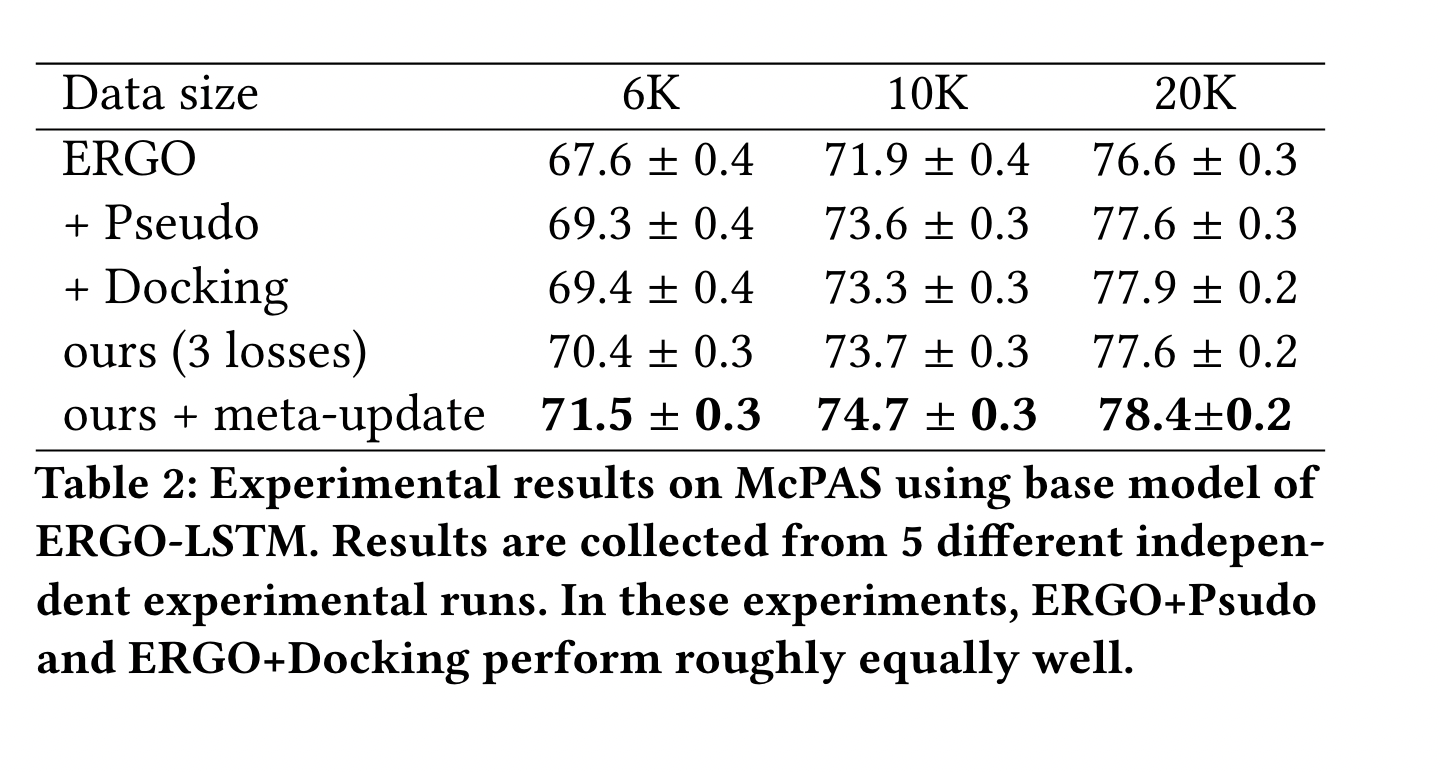
\includegraphics[width=.9\linewidth]{./p5.png}
\end{center}
\end{block}
\end{column}
\end{columns}
\end{frame}

\begin{frame}[label={sec:orgac7d944}]{Results VDJdb}
\begin{columns}
\begin{column}{0.4\columnwidth}
\begin{block}{LSTM}
\begin{center}
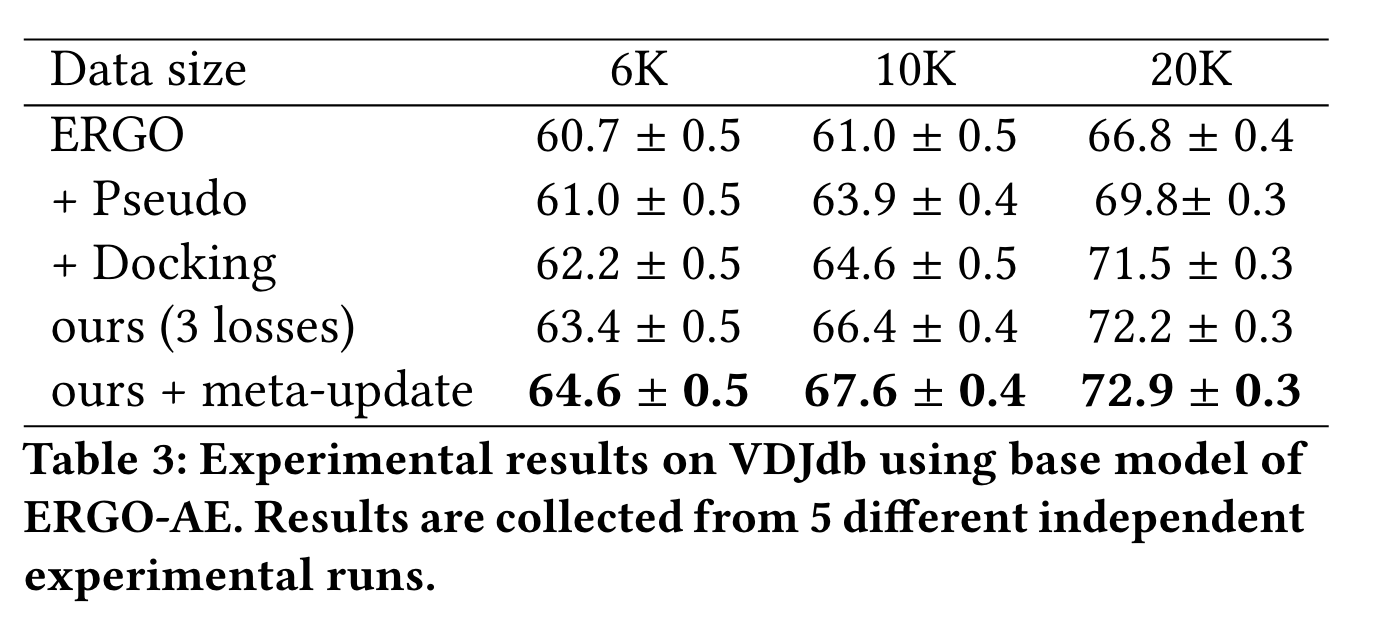
\includegraphics[width=.9\linewidth]{./p6.png}
\end{center}
\end{block}
\end{column}

\begin{column}{0.4\columnwidth}
\begin{block}{AE}
\begin{center}
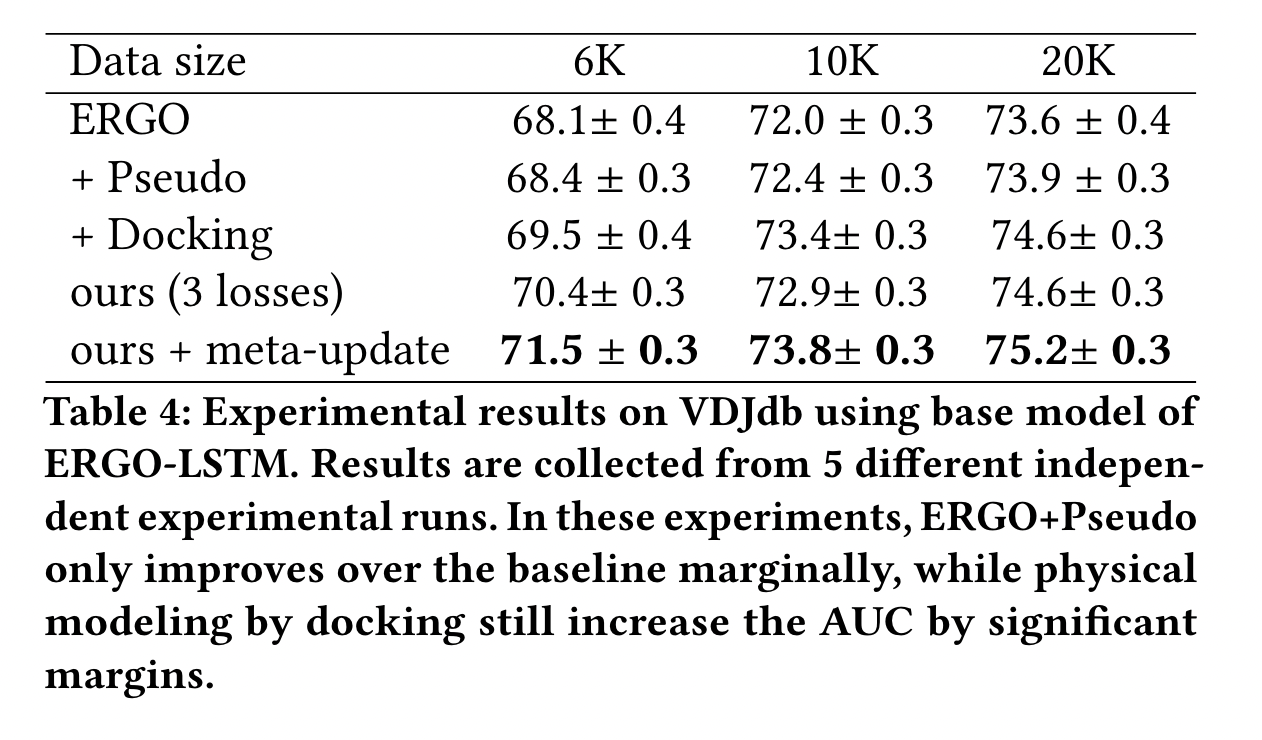
\includegraphics[width=.9\linewidth]{./p7.png}
\end{center}
\end{block}
\end{column}
\end{columns}
\end{frame}

\begin{frame}[label={sec:orgaafa611}]{Results Rare Peptides}
\begin{itemize}
\item A rare peptide KRWIILGLNK has only AUC score of 52.8,
\item while this method achieves 68.1.
\item Note that the average AUC for all peptides is 54.4.
\end{itemize}

\begin{center}
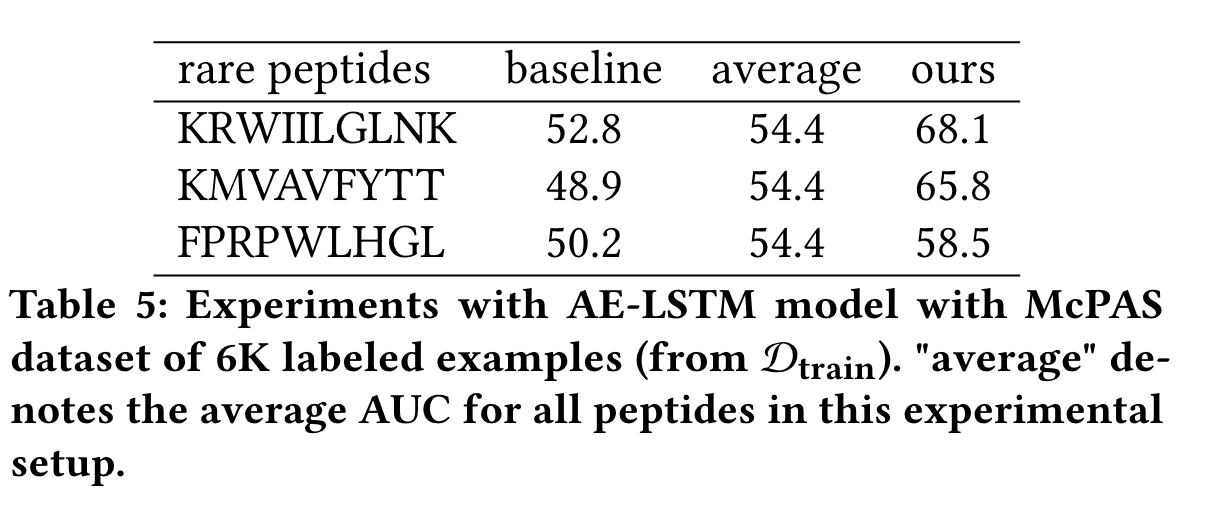
\includegraphics[width=.9\linewidth]{./p8.png}
\end{center}
\end{frame}

\section{Conclusion}
\label{sec:orgb6fd2fc}

\begin{itemize}
\item Goal: Improve the prediction of TCR-peptide interactions
\item Solution:
\begin{itemize}
\item Docking energies as the physical properties between TCR-peptide pairs
\item Data-augmented pseudo-labeling
\item Look ahead meta-update
\item Experiments on VDJdb and McPAS datasets
\end{itemize}
\end{itemize}

\section{References}
\label{sec:org521c989}

\begin{frame}[allowframebreaks]{References}
\printbibliography[heading=none]
\end{frame}
\end{document}